%!TeX program = pdflatex
% Template from: https://github.com/kourgeorge/arxiv-style
\documentclass[a4paper, 10pt]{article}

% Template style
\usepackage{arxiv}

% Language and font packages
\usepackage[english]{babel} 
\usepackage[utf8]{inputenc} % allow utf-8 input
\usepackage[T1]{fontenc}    % use 8-bit T1 fonts
\usepackage{lmodern}
\usepackage[scaled=0.85]{DejaVuSansMono}
\usepackage{microtype}      % microtypography

% Math and values packages
\usepackage{amsmath} 
\usepackage{amsfonts} 
\usepackage{amssymb}
\usepackage{mathtools}
\usepackage{bm}
\usepackage{nicefrac}       % compact symbols for 1/2, etc.
\usepackage[binary-units=true]{siunitx}

% Figures and tables packages
\usepackage{booktabs}       % professional-quality tables
\usepackage{graphicx}
\usepackage{caption} 
\usepackage{subcaption} 
\usepackage{float}
\usepackage[section]{placeins} 

% Miscellaneous
\usepackage{xcolor}
\usepackage{enumitem}
\usepackage{listings}

% Bibliography and reference packages
\usepackage{natbib}
\usepackage[hyphens]{url}           % simple URL typesetting
\usepackage[hidelinks]{hyperref}    % hyperlinks
\usepackage{cleveref}

\lstdefinestyle{json}{
    breaklines=true,
    basicstyle=\small\ttfamily,
    numberstyle=\small\ttfamily,
    numbers=left
    ,xleftmargin=2.5em,
    frame=leftline
    ,tabsize=2
}

\newcommand{\code}[1]{\texttt{#1}}

%%%%%%%%%%%%%%%%%%%%%%%%%%%%%%%%%%%%%%%%%%%%%%%%%%%%%%%%%%%%%%%%

\title{Conversational PEGASUS}

\date{\today}	% Here you can change the date presented in the paper title
%\date{} 					% Or removing it

\author{
	Gonçalo Raposo \\
	\texttt{goncalo.cascalho.raposo@tecnico.ulisboa.pt} \\
	\and
	INESC-ID, Instituto Superior Técnico, Universidade de Lisboa \\[2ex]
	Lisbon, Portugal
}
\renewcommand\footnotemark{}

% Uncomment to override  the `A preprint' in the header
\renewcommand{\headeright}{}
\renewcommand{\undertitle}{}
\renewcommand{\shorttitle}{Dialog Systems Survey}

%%% Add PDF metadata to help others organize their library
%%% Once the PDF is generated, you can check the metadata with
%%% $ pdfinfo template.pdf
\hypersetup{
    pdftitle={Conversational PEGASUS},
    pdfsubject={cs.CL, cs.LG, cs.NE},
    pdfauthor={Luísa Coheur, Gonçalo Raposo, Ricardo Rei, Rui Ribeiro},
    pdfkeywords={First keyword, Second keyword, More},
}

\begin{document}
\maketitle

% Abstract %%%%%%%%%%%%%%%%%%%%%%%%%%%%%%%%%%%%%%%%%%%%%%%%%%%%%

\begin{abstract}

\end{abstract}

% keywords can be removed
\keywords{First keyword \and Second keyword \and More}

%%%%%%%%%%%%%%%%%%%%%%%%%%%%%%%%%%%%%%%%%%%%%%%%%%%%%%%%%%%%%%%%

\section{Motivation}

    PEGASUS is an abstractive summarization model that was proposed in \cite{Zhang2020b}. Given a question, if the passages relevant for the answer are available, then the answering task will be very similar to a summarization of those passages.

\section{Relevant Passages Retrieval}

    A system that given a question, retrieves passages from a database/document/website that are related with the question and are relevant for a possible answer. Use work from Rita Costa.

\section{Answer Generation}
    \subsection{PEGASUS Model}
    
        PEGASUS is an abstractive summarization model that was proposed in \cite{Zhang2020b}. Abstractive summarization differs from extractive summarization in the sense that it might output words or sentences that are not present in the input text. It has a Transformer encoder-decoder architecture, each with 16 layers, and was pre-trained with two objectives:

        \begin{itemize}
            \item Gap Sentences Generation (GSG): Masking whole sentences from a document and generating these gap-sentences from the rest of the document. This works well as a pre-training objective for summarization tasks.
            \item Masked Language Modeling (MSM): Select 15\% tokens in the input text and mask 80\%, replace 10\% by a random token, and 10\% leave unchanged. The decoder has to correct those masked words.
        \end{itemize}

        \begin{figure}[!htb]
            \centering
            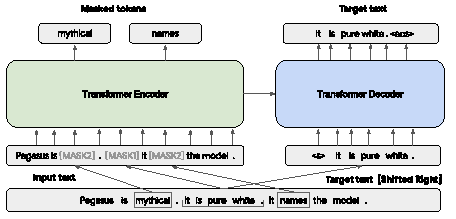
\includegraphics[width=0.8\textwidth]{Figures/pegasus.pdf}
            \caption{Transformer encoder-decoder architecture of PEGASUS model. Both GSG and MLM objectives are represented using the \texttt{[MASK1]} and \texttt{[MASK2]} tokens, respectively. Illustration obtained from \cite{Zhang2020b}.}
        \end{figure}
        
        For pre-training, 2 large text corpus were used: C4 (text from 350M Web-pages), and HugeNews (1.5B articles). This model is able to adapt very quickly when fine-tuning with small numbers of supervised pairs (1000 examples).
        
        Various checkpoints are provided: PEGASUS-large consists in the pre-trained model, and the others (e.g.\ PEGASUS-xsum) correspond to checkpoints that fine-tuned the model with specific datasets (e.g.\ XSum).
        
    \subsection{TREC CAsT Dataset}
        
        The first idea was to use the dataset from TREC CAsT (Conversational Assistance Track) year 2, discussed in \cite{Dalton2020}. Bellow is an alleged example from this dataset:

        \begin{lstlisting}[style=json]
{
  "number": 2,
  "turn": [
    {
      "number": 1,
      "raw_utterance": "What are the main breeds of goat?"
      "system_response": "The main types of goats include..."
      "response_document": "MARCO_5023599"
    },
    {
      "number": 2,
      "raw_utterance": "Tell me about boer goats."
      "system_response": "The development of the Boer goat in the early 1900s can be traced to the Dutch farmers of South Africa. Boer is a Dutch word meaning farmer."
      "response_source": "MARCO_2533087"
    },
    ...
  ],
}
        \end{lstlisting}

        As can be seen above, for each raw utterance, there is a system response and a response document/source. For the example presented, the response document/source, which would correspond to the relevant passage, points to a document from the MS MARCO (Microsoft Machine Reading Comprehension) dataset.

        However, the TREC CAsT dataset turned out not to include the system responses, therefore, it could not be used to train the proposed model.

    \subsection{MS MARCO Dataset}

        MS MARCO (Microsoft Machine Reading Comprehension), presented in \cite{Nguyen2016}, is a large scale dataset. Since its release, currently has $>10^6$ unique real queries from Bing and focus not only in QA but many more problems related to search. Each entry of the MS MARCO dataset has the following structure:

        \begin{lstlisting}[style=json]
{
  "answers": {
    "[]": "string"
  },
  "passages": {
    "[]": {
      "is_selected": "int32",
      "passage_text": "string",
      "url": "string"
    }
  },
  "query": "string",
  "query_id": "int32",
  "query_type": "string",
  "wellFormedAnswers": {
    "[]": "string"
  }
}
\end{lstlisting}

        Given that each sample as a user query, relevant passages, and an answer, maybe this dataset could be used to train the proposed model. However, there is no conversational information.

    \subsection{CoQA Dataset}

        CoQA (Conversational Question Answering) is a large-scale dataset that was proposed in \cite{Reddy2019}. This dataset consists of $>10^5$ question-answer regarding multiple text passages. What distinguishes this dataset is that the questions are conversational and the answers can be free-form text. This dataset has the following structure:
        
        \begin{lstlisting}[style=json]
{
  "data": [
    {
      "source": "mctest",
      "id": "3dr23u6we5exclen4th8uq9rb42tel",
      "filename": "mc160.test.41",
      "story": "Once upon a time, in a barn near a farm house, there lived a little white kitten named Cotton. Cotton ...",
      "questions": [
        {
          "input_text": "What color was Cotton?",
          "turn_id": 1
        },
        {
          "input_text": "Where did she live?",
          "turn_id": 2
        },
        ...
      ],
      "answers": [
        {
          "span_start": 59,
          "span_end": 93,
          "span_text": "a little white kitten named Cotton",
          "input_text": "white",
          "turn_id": 1
        },
        {
          "span_start": 18,
          "span_end": 80,
          "span_text": "in a barn near a farm house, there lived a little white kitten",
          "input_text": "in a barn",
          "turn_id": 2
        },
        ...
    ],
    ...
        \end{lstlisting}

    \subsection{Preparing the Data}

        Given the proposed task, the input of the model will correspond to a question concatenated with the corresponding story. As an example, a sample from the CoQA dataset would be constructed as:
        
        \begin{itemize}
            \item [\underline{Input}:] ``What color was Cotton? \\ Once upon a time, in a barn near a farm house, there lived a little white kitten named Cotton. Cotton ...''
            \item [\underline{Output}:] ``white''
        \end{itemize}
        
        With the input and output defined, the next step is the tokenization, which corresponds to assign a number/id to each token of the text. For this step, there are two memory and performance optimizations that can be performed, namely, choosing an appropriate integer data type and reducing the padding introduced in the batch tensor.

        \subsubsection{Data Type}
        
            To implement the pre-trained PEGASUS model, the Transformers library from Hugging Face was used. More detail can be found in \cite{Wolf2020}. Referring to its documentation\footnote{https://huggingface.co/transformers/}, one can observe that \code{torch.LongTensor} is used for a token ids tensor, which uses long integers for each token id. A long integer occupies 8 bytes = 64 bits, which allows to represent about \num{1.8e19} different tokens. Considering that the vocabulary size of PEGASUS defaults to 50265 tokens, a long integer is unnecessarily large to store PEGASUS tokens. Apart from the \code{MASK} token, the other tokens are a positive integer, therefore, a 32-bit integer is enough for this scenario, since it can represent about \num{2.1e9} positive values. One might wonder if a 16-bit integer would still be enough, but it is only able to represent 32767 positive values, which is insufficient.
            
            Replacing 64-bit integers (long) by 32-bit integers is, therefore, a costless way to reduce the memory utilization of the input and output tensors by half. The task of choosing the appropriate data type considering the representation requirements is an important and beneficial one. However, the model expects the output/labels tensor to be a \code{torch.LongTensor} and raises an error otherwise. This could probably be fixed, but for the current application that tensor was kept as a \code{torch.LongTensor} while the input tensor is reduced to a \code{torch.IntTensor}.
            
        \subsubsection{Dynamic Batches}
        
            The PyTorch Lightning framework, available in \cite{Falcon2019}, was used to train and test the model. The typical pipeline of preparing the dataset consists in reading the text sentences and passing them to the tokenizer, which returns a tensor where each row will correspond to the token ids of a sentence. However, since sentences can have different lengths, the tokenizer pads every sentence to the length of the longest one, can be somewhat wasteful if in the dataset there is a much longer sentence than the rest. Although the padded values are masked by the model, they are still considered in the calculations, which spends computing and memory resources.
            
            For this application, a technique I called dynamic batches, or referred in \cite{Benesty2020} as dynamic/variable length padding, was used to decrease that unnecessary padding. It basically consists in delaying the creation of the tensor, so that, instead of creating a tensor for the entire dataset, only create tensors for the batches\footnote{In this paper, the word batches actually refers to mini-batches.}. This way, instead of ending up with all sentences padded to the length of the longest sentence in the dataset, they are padded to the length of the longest sentence in the considered batch. Therefore, each batch tensor may have a different sequence length. This is particularly useful when there are only a few sentences that are much larger.
            
            A thorough analysis was performed in \cite{Benesty2020}, which observed a 4.7 speedup when using dynamic batches of size 16 on the dataset X-NLI (\cite{Conneau2018}).
    
\section{Results}

    The PEGASUS model (checkpoint pegasus-large) was trained with the CoQA dataset for 2 epochs (early stopping while monitoring the validation loss). The maximum input sequence length was set to 1024 and the maximum output sequence length to 256. The batch size had to be only 2 due to insufficient GPU memory, but it accumulates the gradient of 128 batches during training, so that it is similar to a batch size of 256. The loss and ROUGE values obtained  are presented in \Cref{fig:results}.
    
    \begin{figure}[!htb]
    	\centering
    	\begin{subfigure}[b]{0.49\textwidth}
    		\centering
    		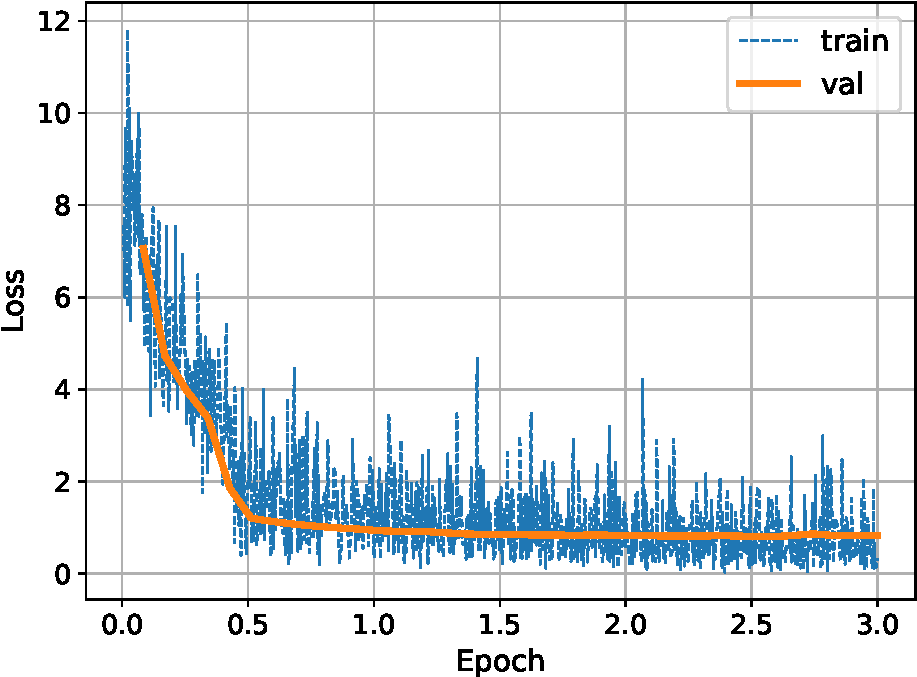
\includegraphics[width=\textwidth]{Figures/loss.pdf}
    		\caption{Train and validation loss.}
    	\end{subfigure}
    	\hfill
    	\begin{subfigure}[b]{0.49\textwidth}
    		\centering
    		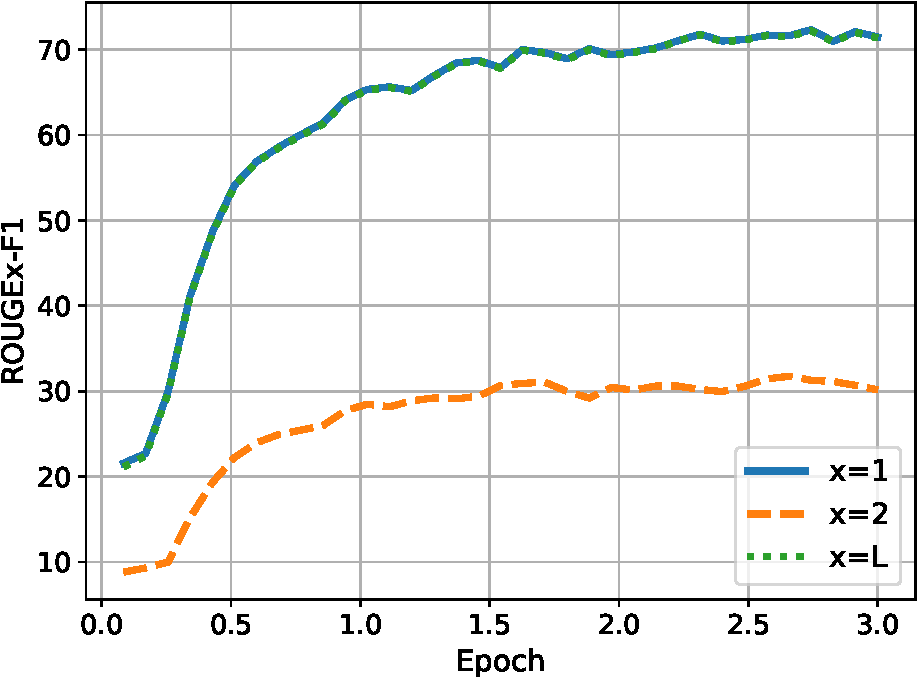
\includegraphics[width=\textwidth]{Figures/rouge.pdf}
    		\caption{ROUGE metric in the validation dataset.}
    	\end{subfigure}
    	\caption{Results of training PEGASUS (large) in CoQA for 2 epochs.}
		\label{fig:results}
    \end{figure}

    \subsection{Interacting with Streamlit}
    
        The best way to validate a conversational QA model is to ask it some questions. In that context, the framework Streamlit\footnote{https://streamlit.io/} was used to design and deploy a simple front-end that would allow to interact with the model by giving a context and questions and then obtaining an answer. The implemented interface is shown in \Cref{fig:streamlit}.A few examples are shown in \Cref{sec:examples}.
        
        \begin{figure}[!htb]
            \centering
            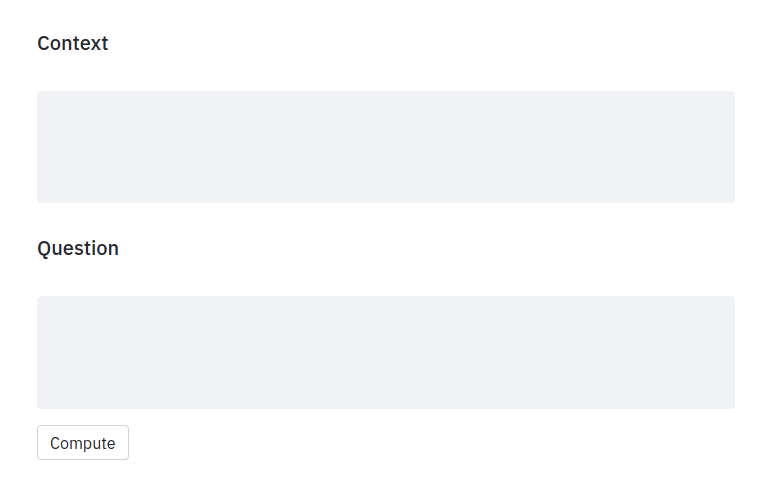
\includegraphics[width=0.6\textwidth]{Figures/streamlit.png}
            \caption{Designed interface using Streamlit.}
            \label{fig:streamlit}
        \end{figure}

%%%%%%%%%%%%%%%%%%%%%%%%%%%%%%%%%%%%%%%%%%%%%%%%%%%%%%%%%%%%%%%%

\clearpage
\bibliographystyle{abbrvnat}
\bibliography{references}      

%%%%%%%%%%%%%%%%%%%%%%%%%%%%%%%%%%%%%%%%%%%%%%%%%%%%%%%%%%%%%%%%

\clearpage
\appendix

\section{Examples from Streamlit}
\label{sec:examples}

    \begin{figure}[!htb]
        \centering
        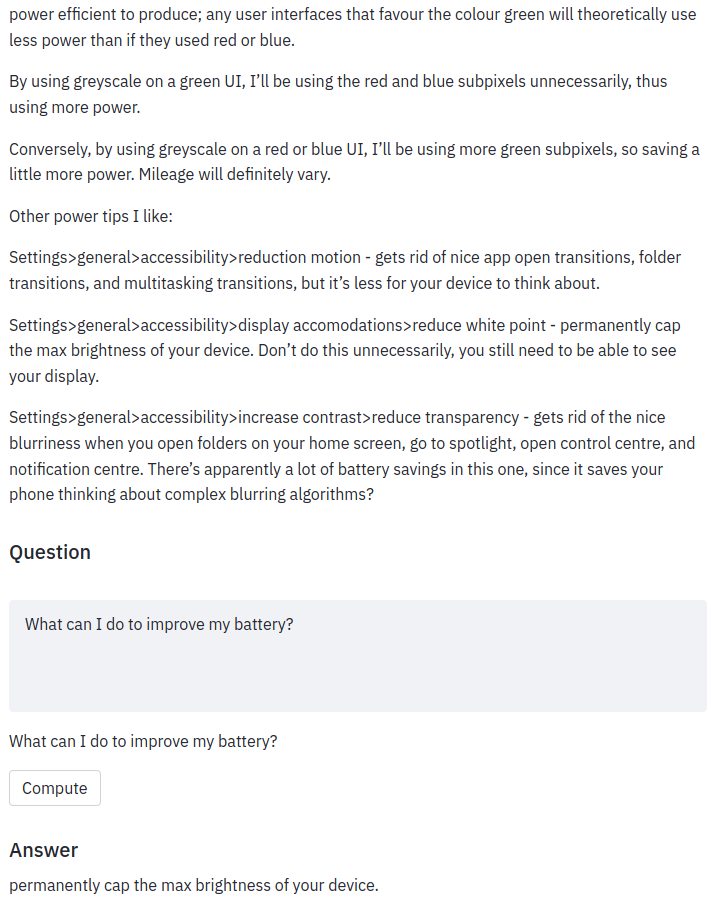
\includegraphics[width=0.8\textwidth]{Figures/battery.png}
        \caption{The context is a set of several tips about improving the battery life of an iPhone.}
    \end{figure}
    
    \begin{figure}[!htb]
        \centering
        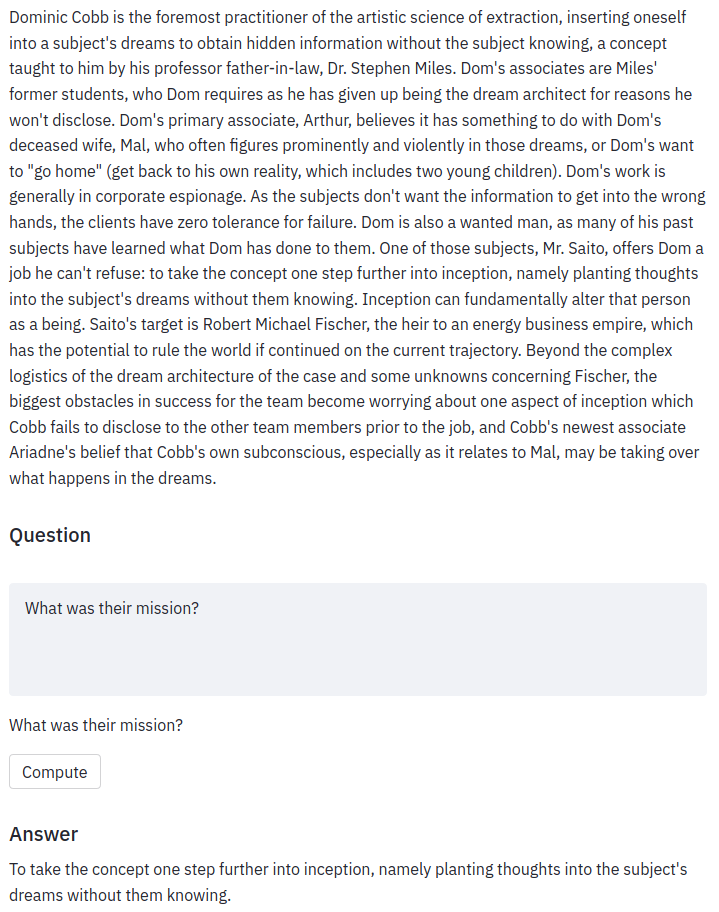
\includegraphics[width=0.8\textwidth]{Figures/inception.png}
        \caption{The context is a synopsis of the movie Inception.}
    \end{figure}
    
    \begin{figure}[!htb]
        \centering
        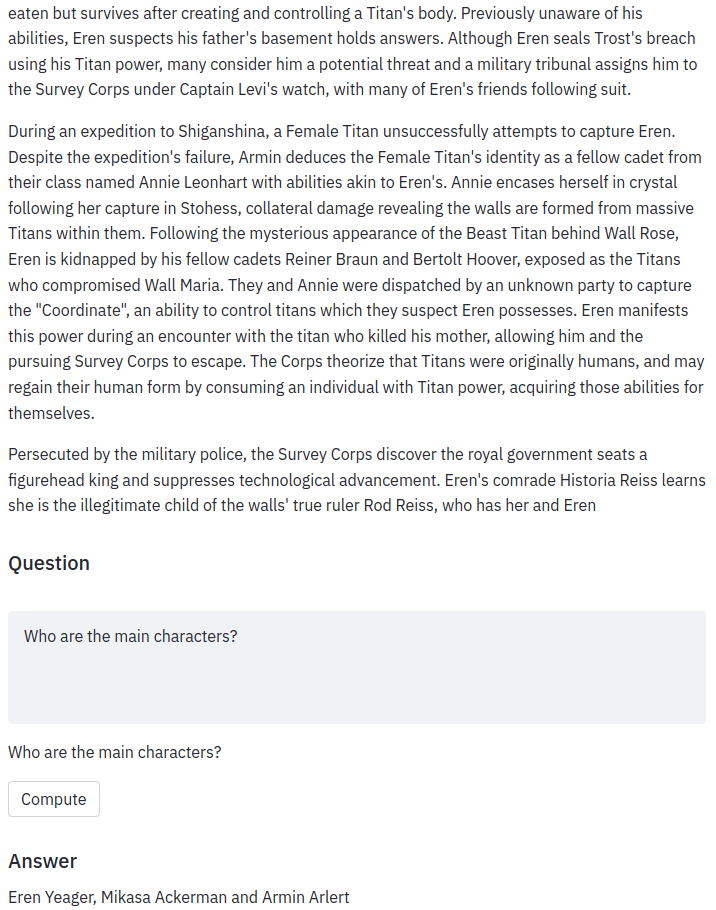
\includegraphics[width=0.8\textwidth]{Figures/attack_on_titan.png}
        \caption{The context is a synopsis of the anime Attack on Titan.}
    \end{figure}
    



\end{document}
